\documentclass[10pt]{book}
\usepackage[utf8]{inputenc}
\usepackage[italian]{babel}
\usepackage{multicol}
\usepackage[bookmarks]{hyperref}
\usepackage[a4paper, total={18cm, 25cm}]{geometry}
\usepackage{listings}
\usepackage{graphicx}
\usepackage{makecell}
\graphicspath{ {./img/} }
\usepackage{color}

\begin{document}
\renewcommand*\contentsname{Indice}
\title{Sviluppo Applicazioni Mobili}
\author{Federico Matteoni}
\date{A.A. 2019/20}
\maketitle
\tableofcontents
\pagebreak
\section*{Introduzione}
Vincenzo Gervasi, \texttt{gervasi@di.unipi.it}\\
\texttt{circe.di.unipi.it/~gervasi/main/}\\
\texttt{developer.android.com}

\paragraph{Modalità d'esame} Sviluppo di un'app, proposta dallo studente ma concordata con il docente. Presentazione dell'app con ispezione del codice e domande "teoriche" su aspetti non coperti dal progetto. No compitini.\\
3 criteri: applicazione mobile, non deve avere senso su applicazione web o su computer. diversità, almeno tre framework presentati. progetto adeguato a esame di 6 CFU.

\chapter{Programmazione Android}
\section{Breve Storia di Android}
\paragraph{2007} Telefonini Nokia, Palm, Windows CE e BlackBerry. Tutti \textbf{sistemi fortemente proprietari}, spesso con versioni frammentate e di difficile manutenzione. Giravano su una versione di Java portatile ma fortemente limitata, \textbf{JavaME}.
\subparagraph{Novembre 2007}  La \textbf{Open Handset Alliance}, formata da vari produttori di telefoni, pubblica la \textbf{Open Platform for Mobile Handset}.\\
Era il 5 Novembre, \textbf{7 giorni dopo rilasciano Android}.\\
Chi c'era dietro, tra le altre: Google, eBay, China Mobile, HTC, Intel, LG, Motorola, NTT DoCoMo, Qualcomm, nVidia, Samsung, Sprint Nextel, Telecom Italia, Telefònica, Texas Instrument, T-Mobile. Ovvero vari produttori di telefoni, di chip, fornitori di servizi e di telefonia.
\paragraph{Android} Il 12 Novembre viene rilasciato \textbf{Android}\\
Rilasciato su licenza Apache, \textbf{basato su Linux 2.6} e sviluppato su Eclipse, Java e Python. Il kernel \textbf{era completo e standard}, non era personalizzato.\\
Sviluppato da \textbf{Android Inc.}, startup californiana nata nel 2003 a Palo Alto, acquistata da Google nel 2005 e brevetti registrati nel 2007. Lo sviluppo è avvenuto in gran segreto, brevetti registrati all'ultimo così da non destare sospetti a Microsoft e Apple. Fondata da \textbf{Andy Rubin}.
\subparagraph{Adesso} Dal 2007 sono state rilasciate numerose \textbf{versioni}, dai \textit{codename} ispirati a nomi di dolciumi in ordine alfabetico\ldots fino ad Android Q. Adesso parleremo principalmente di software, ma non bisogna dimenticare il lato \textbf{hardware}: potenza di calcolo, efficienza della batteria, sensori e schermi. I produttori, inoltre, hanno \textbf{poco interesse ad aggiornare i telefoni vecchi}: il principale problema è che per ogni modello e ogni aggiornamento bisogna far omologare e convalidare la parte telefonica, quindi servono mesi di test e tanti soldi. Per cui è meglio \textbf{spingere gli utenti a comprarne di nuovi $\Rightarrow$ \textit{frammentazione}}.
\paragraph{Software} Ogni versione è (\textit{quasi}) sempre \textbf{pienamente compatibile con le precedenti}: i cambiamenti nelle API sono identificati da un \textbf{API Level}.\\
Le applicazioni possono quindi dichiarare:
\begin{list}{}{}
	\item \textbf{API Level minimo} di cui hanno bisogno per funzionare
	\item \textbf{API Level targe} per cui sono state scritte
	\item \textbf{API Level massimo} oltre il quale non funzionano più (pessima idea, sconsigliato, obsoleto e ignorato già da Android 2.0.1)
\end{list}
I vincoli vengono verificati dal market e dalle procedure di aggiornamento del S.O.\\\\
Rispetto iOS, i quali dispositivi vengono (\textit{quasi}) sempre aggiornati alla versione più recente, Android tende a diffondere gli aggiornamenti più lentamente: l'Android più recente è sempre una nicchia.\\
\paragraph{Supporto} Google cerca di supportare più o meno all'infinito le vecchie versioni del S.O. con le \textbf{librerie di compatibilità} (\texttt{libcompat}).
\begin{list}{}{}
	\item Codice che le applicazioni possono includere nel loro "eseguibile"
	\item Simula le funzioni delle versioni più recenti sulle versioni più vecchie
\end{list}
Inoltre, parte delle funzioni del S.O. sono incorporate nei \textbf{Google Play Services}, libreria aggiornabile dal market.\\
Un \textbf{grosso ostacolo} è la \textbf{customizzazione} (skinning) del sistema.

\section{Ant e Gradle}
Ant antiquato\\
Gradle più moderno.
\paragraph{Gradle} Sistema di build avanzato, configurabile. Distribuito nel senso di risorse per lo sviluppo sparse in rete tramite URL. Fill-in del manifest (manifest contiene metadati per il s.o.), gradle genera e mantiene aggiornato il manifest.\\
\\
\texttt{compileSdkVersion} per fill-in manfest e \texttt{buildToolsVersion} per scaricare tools se non presenti.\\
\texttt{Lint} analisi statica di codice per warnings e errori sintattici della scrittura del codice.\\\\
\section{Architettura Android Studio/Gradle}
IntelliJ con plugin: android plugin. android designer, android gradle adapter.\\
Si appoggia all'android SDK e a Gradle (tool separato, con plugin android e anch'esso collegato all'SDK)\\
Inoltre c'è il progetto, con \texttt{.properties} con config per l'ambiente di sviluppo (come dove si trova il compilatore ecc.) e \texttt{build.gradle}.

\chapter{Architettura Android}
\begin{center}
	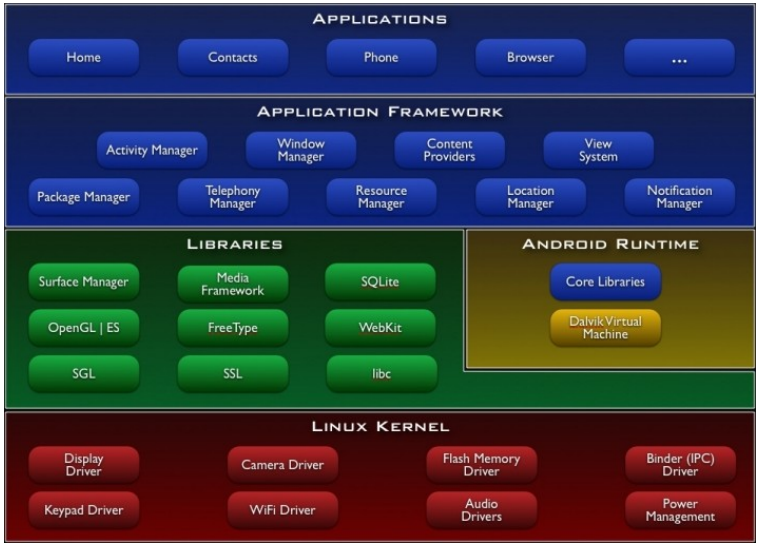
\includegraphics[scale=0.7]{arch_thebigpicture.png}
\end{center}
Studieremo a fondo le \textbf{applicazioni} e parte dell'\textbf{Android Runtime}. Le \textbf{libraries} sono largamente invisibili e il \textbf{linux kernel} è utile da sapere.
\section{Struttura}
\textit{Bottom -- Up}
\paragraph{Kernel Linux} Alla base di tutto c'è il \textbf{kernel Linux standard, senza personalizzazioni}. Gli \textbf{adattamenti} per la parte telefonica sono \textbf{eseguiti tramite moduli del kernel}. Come display driver, driver per la tastiera keypad, driver camera, wifi, memoria flash, audio, driver binder (IPC) che cura Inter-Process Communication (diversamente da socket e FIFO, che non andavano bene per Android. \textbf{Su Android non ci sono solo file, ma oggetti con metodi}, e FIFO/socket adatte per trasferire flussi di byte. Il \textbf{binder fa comunicare processi in termini object-oriented}). Per ultimo c'è il power management driver.\\
Per il resto è il kernel linux tanto conosciuto e amato: utenti, diritti, shell, librerie, thread e comandi.
\paragraph{Librerie} Librerie \texttt{.so}, che fanno tantissime cose. Tra esse ci sono: surface manager (equivalente dei window system X o wayland), OpenGL ES per la grafica 3D, FreeType, SSL (HTTPS e Secure Socket Layer), WebKit, SQLite, libc (scanf, strlen\ldots).
\subparagraph{Android Runtime} In aggiunta alle librerie, c'è anche la \textbf{Macchina Virtuale che esegue il codice delle applicazioni Android} (\textbf{Dalvik}/\textbf{ART}), insieme alle core libraries (garbage collector, heap, memoria\ldots)
\paragraph{Separazione tra mondo Java e mondo del codice eseguibile ARM} Da qui in poi c'è il linguaggio Java, fin'ora il linguaggio (del kernel linux) è il C.
\paragraph{Application Framework} S.O. rappresentato da oggetti nello heap. Librerie: package manager, telefony manager, activity manager, window manager, location manager (GPS), notification manager
\paragraph{Applicazioni} Tra cui servizi interni: home, contatti, telefono, browser\ldots Firmate a chiave asimmetrica. Platform key per applicazioni che usano funzioni critiche, chiave che firma il kernel.
\section{Dalvik \& ART}
\paragraph{Dalvik} La stragrande maggioranza delle applicazioni gira su una macchina virtuale: \textbf{Dalvik}. Funziona in maniera analoga alla JVM con importanti differenze:
\begin{list}{}{}
	\item Basata su \textbf{registri} e non su stack
	\item \textbf{Set di istruzioni ottimizzato} per risparmiare memoria e aumentare la velocità d'esecuzione
	\item \textbf{Formato dei file eseguibili ottimizzato} per risparmiare memoria
	\item \textbf{Eseguibile da più processi con una sola istanza}: tutto \textbf{codice rientrante} e sharing del codice di Dalvik via \texttt{mmap()}.
	\item \textbf{Non} sotto il controllo di Oracle (storica causa legale)
\end{list}
\paragraph{Due meccanismi} Fino ad Andorid 4.3 l'unico meccanismo di esecuzione era Dalvik. Durante Android 4.4 si è aggiunta l'opzione per eseguire su ART, con Dalvik come opzione default.\\
Da Android 5 in poi si esegue su ART.
\paragraph{Android Runtime} ART ha delle differenze importanti rispetto ha Dalvik:
\begin{list}{}{}
	\item ART \textbf{pre-compila a install-time}, non interpreta\\
	Questo rende l'installazione più lenta, ma l'\textbf{esecuzione più veloce}
	\item Processo largamente \textbf{invisibile} a programmatore e utente
	\item Però utilizzano lo stesso bytecode, producendo però \textbf{codice nativo} invece che bytecode: ulteriore assicurazione contro le cause di Oracle
\end{list}
\paragraph{Entrambi rilevanti} Dalvik e ART sono entrambi rilevanti perché
\begin{list}{}{}
	\item Dalvik perché è il target della toolchain di compilazione del 99\% delle app
	\item ART perché Google da tempo sviluppa e supporta soltanto questa:
	\begin{list}{}{}
		\item Più veloce in esecuzione
		\item Miglior gestione della garbage collection
		\item Maggiore integrazione con profiling e debugging
		\item Minor consumo di energia
	\end{list}
\end{list}
\begin{center}
	\begin{tabular}{ p{4 cm} | p{5 cm} | p{5 cm}}
	\textbf{Fase} & \makecell{\textbf{Dalvik}} & \makecell{\textbf{ART}} \\
	\hline
	Compile-Time & \makecell{\textbf{javac}: \texttt{.java} $\rightarrow$ \texttt{.class}\\\textbf{dx}: \texttt{.class} $\rightarrow$ \texttt{.dex}} & \makecell{\textbf{javac}: \texttt{.java} $\rightarrow$ \texttt{.class}\\\textbf{dx}: \texttt{.class} $\rightarrow$ \texttt{.dex}} \\
	\hline
	Install-Time & \makecell{\textbf{dexopt}: \texttt{.dex} $\rightarrow$ \texttt{.odex}} & \makecell{\textbf{dex2oat}: \texttt{.dex} $\rightarrow$ \texttt{ELF}} \\
	\hline
	Run-Time & \makecell{\textbf{libdvm.so}: \texttt{.odex} $\rightarrow$ run\\Interpretato + JIT} & \makecell{\textbf{libart.so}: \texttt{ELF} $\rightarrow$ run\\Esecuzione nativa con un po' di\\runtime}
	\end{tabular}
\end{center}
\textbf{JIT} $=$ \textbf{Just-In-Time} compilation, compila pezzi di codice che interpreta più volte
\pagebreak
\subsubsection{Esecuzione}
Ogni app viene eseguita dal kernel Linux
\begin{list}{}{}
	\item \textbf{In un processo separato}, che esegue Dalvik che esegue il bytecode dell'app: \textbf{controllo i permessi d'accesso alle risorse logiche fatto dalla VM} (permessi concessi dall'utente)
	\item \textbf{Con uno user ID distinto}: tutti i file creati dall'applicazione appartengono al proprio user ID, quindi altre applicazioni \textbf{non possono accedere} alla sua directory né \textbf{leggere i suoi file}. Applicazioni "\textit{amiche}" (specificato nel \texttt{Manifest}) possono condividere processo e user ID, ma devono avere la stessa firma.\\
	Il \textbf{controllo dei diritti di accesso alle risorse fisiche è fatto dal kernel} (i diritti \textbf{non} sono controllati dall'utente)\\
	Riferisce la singola installazione sulla singola macchina.
\end{list}
\textbf{Disaccoppiamento fra processo e programma}. Il processo è un flusso di esecuzione dell'applicazione, ma \textbf{essa esiste indipendentemente dal processo}. Lo stesso processo può eseguire applicazioni diverse, la stessa applicazione può essere eseguita da processi diversi in momenti diversi.
\paragraph{Risultato} Si ha un notevole grado di \textbf{separazione} e \textbf{isolamento} delle app, anche se ci possono essere sempre bug non scoperti all'interno del kernel Linux.\\
Android è un sistema piuttosto \textbf{sicuro agli attacchi}, eccezione fatta per quelli di ingegneria sociale: un utente può concedere dei permessi ad un'app malevola che li usa per scopi diversi da quelli pubblicizzati.
\paragraph{Utente} L'utente non fa niente, se non tramite le app: non ha un user ID, non è proprietario di nessun file né titolare di nessun processo, non ha nemmeno delle credenziali di login.
\chapter{Struttura di un'App Android}
\paragraph{Diverse forme} Durante la sua vita un'applicazione assume diverse forme:
\begin{list}{}{}
	\item \textbf{Sviluppo}, layout su disco sottoforma di \textbf{progetto}
	\item \textbf{Deployment}, formato dei file \texttt{.apk}
	\item \textbf{Esecuzione}, struttura in \textbf{memoria}
\end{list}
Le varie forme sono legate da tre processi:
\begin{list}{}{}
	\item \textbf{Build}: sorgente $\rightarrow$ \texttt{.apk}
	\item \textbf{Deploy}: \texttt{.apk} su un canale di distribuzione (market\ldots) $\rightarrow$ \texttt{.apk} sul device
	\item \textbf{Run}: \texttt{.apk} $\rightarrow$ processo \textbf{in memoria}
\end{list}
\section{Progetto}
Un'applicazione in sviluppo è un \textbf{progetto}: lo scheletro viene creato automaticamente dal wizard di creazione di un nuovo progetto e \textbf{solo alcune directory sono interessanti per lo sviluppatore} mentre altre sono generate automaticamente.
\subsection{Android Studio}
\begin{list}{}{}
	\item \textbf{manifests}
	\begin{list}{}{}
		\item \texttt{AndroidManifest.xml}: metadati dell'applicazione
	\end{list}
	\item \textbf{java}: sorgenti (\texttt{.java}, \texttt{.kt} e unit test associati)
	\item \textbf{assets}: file arbitrari aggiunti all'\texttt{.apk}
	\item \textbf{bin}: risultato della compilazione (risorse, \texttt{.dex}, \texttt{.apk}\ldots)
	\item \textbf{res}: risorse note al runtime Android
	\begin{list}{}{}
		\item \textbf{animator}: animazioni basate su proprietà
		\item \textbf{anim}: animazioni basate sull'intercalazione
		\item \textbf{color}: colori
		\item \textbf{drawable}: immagini raster o vettoriali
		\item \textbf{layout}: descrizioni dei layout della UI
		\item \textbf{menu}: menù usati dall'app
		\item \textbf{raw}: file arbitrari, alternativa ad \textbf{assets}
		\item \textbf{values}: costanti (stringhe, interi, array\ldots)
		\item \textbf{xml}: file XML arbitrari, incluse le configurazioni
	\end{list}
	\item \textbf{libs}: librerie native custom
	\item \textbf{Gradle Scripts}: configurazioni di build
	\item \textbf{Altri} come \texttt{*.properties}, \texttt{*.cfg}, \texttt{*.xml}\ldots: configurazioni varie
\end{list}
\subsection{Struttura di un progetto}
La struttura vista è quella tipica di un'applicazione. Esistono altre due forme di progetto Android:
\begin{list}{}{}
	\item \textbf{Libreria}, contenente componenti destinati ad essere usati da altre app. In questo modo i membri di una famiglia di app correlate possono condividere componenti. Ogni libreria può essere usata da varie app e ogni app può usare varie libreria.
	\item \textbf{Progetto test}, contenente codice usato per fare il testing di un'altra app.
\end{list}
\section{APK}
\subsection{Contenuti di un APK}
Il \textbf{build} di un'app Android produce un file in formato \texttt{.apk}, che non è altro che una \textbf{specializzazione di uno \texttt{.jar}} (che a sua volta è una specializzazione di uno \texttt{.zip}).
\begin{list}{}{Contenuti:}
	\item \texttt{resources.arsc}, file binario contenente la tabella che mappa ID a risorse
	\item \texttt{classes.dex}: tutti i \texttt{.class} dell'app, convertiti in DEX e unificati in un unico file
	\item \texttt{AndroidManifest.xml}, il manifesto
	\item \textbf{res/*}, file delle risorse
	\item \textbf{META-INF/*}, contenente i certificati pubblici (chiavi), solo per le app firmate
	\begin{list}{}{}
		\item \texttt{META-INF/MANIFEST.MF} che contiene \textbf{informazioni di versionamento} e un \textbf{checksum di ciascun file}
		\item \texttt{META-INF/CERT.*}, certificati RSA\\
		Per il deploy è \textbf{necessario creare un proprio certificato}, quello di debug è generato da ADT
	\end{list}
\end{list}
Un \texttt{.apk} è dunque un \textbf{archivio contenente tutti i componenti di un app}:
\begin{list}{}{}
	\item \textbf{Auto-descrittivo} grazie ai manifesti
	\item \textbf{Compatto} grazie alla compressione
	\item \textbf{Affidabile} grazie alla firma digitale: non è possibile aprire un \texttt{.apk}, sostituire alcuni componenti e re-impacchettarlo perché \textbf{la firma sarebbe invalidata}
	\item Facilmente \textbf{distribuibile} perché è un file unico
	\item Facilmente \textbf{installabile}, niente wizard di installazione\\
	In \textbf{/sys/app} se preinstallata o in \textbf{/data/app} se installata dall'utente
\end{list}
\pagebreak
\section{Memoria}
\subsection{Struttura in memoria}
Una volta caricata in memoria un'app si distingue in \textbf{componenti}. Solitamente 1 app $=$ 1 processo $=$ 1 VM $=$ 1 thread, ma possibili variazioni: multithread, app amiche sullo stesso processo\ldots\\
Il flusso di lavoro dell'utente (\textbf{task}) è spesso fatto di componenti appartenenti ad app diverse, su processi diversi. Android \textbf{incoraggia la condivisione sicura fra app} sia di dati che di componenti $=$ funzionalità.
\begin{center}
	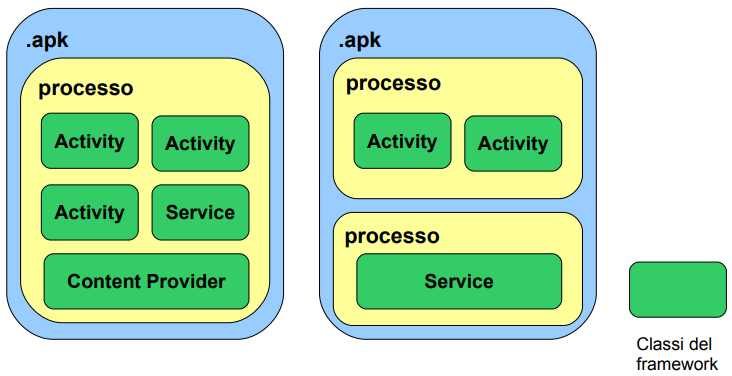
\includegraphics[scale=0.7]{strutturamem.png}
\end{center}
L'app a sinistra, per esempio, è formata da 5 componenti.
\begin{list}{}{I componenti che vedremo durante il corso possono essere dei seguenti \textbf{tipi}:}
	\item \textbf{Activity}: una "schermata" dell'app
	\item \textbf{Content Provider}: un fornitore di dati condivisi
	\item \textbf{Service}: un fornitore di servizi condivisi (senza UI)
\end{list}
Un \textbf{task}, cioè quello che vede l'utente, può essere formato da un'activity dell'app a sinistra e le due activity dell'app a destra. C'è quindi una \textbf{importante distinzione} tra le visioni di programmatori e utenti:
\begin{list}{}{}
	\item un programmatore percepisce come "app" un \texttt{.apk}
	\item un utente percepisce come "app" un \textbf{task}.
\end{list}
Quindi per garantire una UX gradevole occorre che l'integrazione sia \textbf{seamless}: uso di stili, temi e icone simili (\textbf{style guide}), \textbf{consistenza fra le app} più importante della consistenza dentro le app o fra piattaforme
\section{Navigazione}
Navigazione: utente passa da un contesto all'altro. Navigazione gerarchica, posso dal task leggere una mail e tornare indietro o andare a leggere il resto delle mail.\\
Originariamente solo tasto back, stack push e pop. Per lungo tempo ha asservito agli scopi, ispirato al paradgima navigaz web. Poi non era più sufficiente. Porta a sistemi nato per esser epiù logico ma confonde di più. Attualmente almeno due diverse: tasto back risale stack attività dove sono stato (Schermata in cui ero prima) e tasto up torna a livello logico superiore di dove  sono (non è detto che ci sia già stato, solitamente implementato come icona nella actionbar).\\
Caso tipico è navigazione con pattern master-detail. Classico pattern di progettazione app. Pattern: soluzione adattabile per problemi frequenti. Nel master detail problema generale è: ho lista di cose e poi ho dettagli su quelle cose. Elenco mail ma posso leggerle, elenco chat ma posso entrare nella chat.
\chapter{Risorse}
%http://circe.di.unipi.it/~gervasi/SAM19/Lezione%2002-03.pdf, 39 [25/02 1h 02]
\section{Accesso alle Risorse}
Ho risorse nella cartella res organizzate. Produce classe R.java che dà nomi usabili tipati. Efficienza perché uso interi per riferire oggetti di vari tipi (layout, stringhe\ldots) che non vengono creati sullo heap. Al tempo stesso controllo staticamente tipi a seconda di R.layout, R.string\ldots Così alloco gli oggetti solamente quando servono, all'ultimo momento.\\
Accesso alle risorse metodi della classe \texttt{Context}, superclasse dei \texttt{Component}. Ogni pezzo dell'app è un context, da un thread, in una classe, in un'app, eseguita forse da un processo. \texttt{Context.getResources().get}\ldots\texttt{(int id)}. Ci sono anche metodi per accedere alle risorse \texttt{raw} (risorse di tipo non interpretabile dal sistema): \texttt{InputStream openRawResource(int id)}\\
\texttt{AssetManager getAssets()} l'asset manager sola letture legge file: list lista file, assetfiledescriptor: file da usare in contesto più posix, magari per passarlo a metodo nativo scritto in C o a decoder assembler e inputstream: file da leggere ancora nel mondo java wrapper decode\ldots\\
\subsection{Risorse alternative} Per un certo numero di condizioni dell'ambiente si può indicare quali risorsi usare in che contesto: lingua, dimensioni schermo\ldots\\
ID risorse è identificatore logico. Alcuni esempi\ldots\\
Questo è fatto tramite qualificatori che descrivono aspetti dell'ambiente, si affiancano alle sottodirectory di res: \texttt{res/tipo-qualificatori}. Es \texttt{res/drawable-ja} icone da usare su dispositivi in lingua giapponese. \texttt{drawable-ldpi}, \texttt{drawable-hdpi}\\
\ldots carellata qualificatori\ldots
Runtime processo di scelta.
processo di scarto rimango con più opzioni scelgo quella per priorità, rimango con una ad un certo punto scelgo quella, rimango con 0. Se nessuna matcha tutti validi, se ne matcha una o più scarto i non validi. Inoltre c'è directory di default.
\chapter{Componenti di un'app Android}\section{Ciclo di Vita}
Tipicamente un'app Android esegue così
\begin{list}{}{}
	\item Il launcher (che è esso stesso un'Activity) avvia la prima Activity dell'app \textbf{inviandole un'Intent} che indica l'intenzione di lanciarla. L'activity chiama \texttt{setLayout()} per impostare la propria UI
	\item Il sistema chiama certi metodi dell'Activity (\textbf{callback}) in risposta alle azioni dell'utente\\
	A seconda dei casi, questi metodi potranno
	\begin{list}{}{}
		\item Lanciare altre Activity (inviando opportuni Intent), sia dell'app che di altre app
		\item Inviare Intent ad Activity già in esecuzione o in broadcast a tutti gli interessati
		\item Interagire con Services in background
		\item Recuperare o salvare dati tramite un Content Provider
		\item Terminare l'Activity, tornando alla precedente
	\end{list}
\end{list}
\section{Componenti}
\paragraph{Cooperazione} Abbiamo visto che le applicazioni Android non sono un blocco monolitico ma un insieme di componenti cooperanti:
\begin{list}{}{}
	\item \textbf{Activity}\\
	Compone un'attività atomica dell'utente, concretizzata in una "\textbf{schermata}". Può essere \textbf{composta} da vari \textbf{Fragment}
	\item \textbf{Service}\\
	Attività di sistema o dell'app \textbf{invisibile all'utente}, eseguita in background. \textbf{Non interagisce con l'utente} ma \textbf{può interagire con le applicazioni} in vari modi.
	\item \textbf{Content Provider}\\
	Un componente che \textbf{pubblica "contenuti"}, con un'interfaccia programmatica che viene utilizzata da altre app.
	\item \textbf{Broadcast Receiver}\\
	"\textbf{Ascolta}" i messaggi \textbf{globali}. Quando riceve un messaggio di suo interesse, esegue del codice specifico (ad esempio, lancia un'attività).
\end{list}
\subsection{Intent}
I vari componenti \textbf{dialogano attraverso un sistema di messaggistica} che è alla base di Android
\paragraph{Intent} Un Intent è un \textbf{messaggio} che \textbf{esprime un'intenzione di un utente o un'app affinché avvenga qualcosa}.\\
Ci sono numerosissimi intent di sistema, ma ogni app può definirne altri. Una \textbf{parte della struttura} del messaggio \textbf{è fissata}, ma possono \textbf{includere dati "extra" a piacere}.\\
Gli intent possono essere \textbf{indirizzati ad uno specifico componente} oppure \textbf{emessi in broadcast}.\\
Ogni app definisce un \textbf{filtro} che \textbf{dichiara a quali intent è interessata} e può eventualmente rispondere.

\pagebreak
Per \textbf{avviare un'Activity} ci sono due modi
\begin{multicols}{2}
\begin{list}{}{}
	\item \textbf{Explicit Intent}: possiamo creare un Intent che \textbf{chiede un'Activity}.\\
	Se l'Activity in questione non è in esecuzione allora viene lanciata.\\
	Se è già in esecuzione viene "svegliata".\\
	In entrambi i casi, viene recapitato l'Intent e l'Activity destinataria diventa "attiva".
	\columnbreak
	\item \textbf{Implicit Intent}: possiamo creare un Intent che \textbf{chiede una funzione}.\\
	Il \textbf{sistema cerca quale Activity può rispondere}. Se ne trova una, la attiva.\\
	Se ne trova più di una, chiede all'utente quale lanciare.\\
	Se non ne trova nessuna, fallisce.
\end{list}
\end{multicols}
\paragraph{Esempio di Implicit Intent} \texttt{ACTION\_SEND}. L'app crea un Intent implicito con \texttt{ACTION\_SEND}, ci mette dentro i dati da inviare e lo affida al sistema che cercherà le app installate che supportano \texttt{ACTION\_SEND} e chiederà all'utente quale usare.
\subsection{Contenuti di un Intent}
\begin{list}{}{}
	\item \textbf{Action}: quale azione si vuole ottenere (\texttt{String})
	\item \textbf{Data}: su quale dato operare (\texttt{URI})
	\item \textbf{Type}: tipo MIME di Data (\texttt{String})\\
	Se non è fornito viene ricavato da Data, se è fornito fa override su quello di Data.
	\item \textbf{Component}: componente a cui è indirizzato il messaggio.\\
	Solo per Intent espliciti
	\item \textbf{Extras}: un \texttt{Bundle} (mappa chiave $\rightarrow$ valore) di ulteriori campi
	\item \textbf{Flag}: \ldots
\end{list}
\subsection{Intent Filter}
%http://circe.di.unipi.it/~gervasi/SAM19/Lezione%2004-05.pdf p.14, h 16:13 

\subsection{Activity Stack}
Utente interagisce solo con la top ma può vedere le altre parti se la top ha parti trasparenti.\\
Ci sono tanti stack. In un dato momento sono in uno stack. Se scelgo di cambiare schermata vado sull'activity precedente a questa in ordine cronologico sempre sul suo stack.\\
Politica con cui vengono avviate activity\ldots (p.36)\\
Comportamento dipende da due flag: uno deciso da chi manda l'activity e altri flag decisi dall'activity.\\
\begin{list}{}{\texttt{launchMode} (manifest)}
	\item \texttt{Standard} crea sempre nuova istanza
	\item \textbf{SingleTop} riavvia istanza se activity top altrimenti nuova istanza che diventa top
	\item \textbf{SingleTask} Una sola istanza, se ce n'è una in qualche stack viene riavviata quella altrimenti nuovo stack
	\item \textbf{SingleInstance} Si crea nuobo task che non consente altre activity (es.: Home)
\end{list}
Con i \texttt{FLAG\_ACTIVITY\_*} ci sono ulteriori opzioni per essere più specifici
\begin{list}{}{}
	\item Disattivare l'animazione di transizione
	\item Lanciare senza che appaia nella history
	\item Decidere se spostare l'activity in cima allo stack o lasciata al suo posto
	\item \ldots
\end{list}
\begin{list}{}{Flag più comuni (intent)}
	\item new\_task
	\item 
\end{list}
\subsection{Lanciare activity}
Mai usare \texttt{on<qualcosa>} nel codice scritto da noi, sono chiamate fatte dal sistema.
\subsection{Layout}
Il layout è impostato con \texttt{setLayout()}, ma può cambiare dinamicamente: alterando il layout o manipolando i fragment che compongono l'activity.\\
Nel secondo caso i cambiamenti ai fragment vengono messi nel back stack.
\subsection{Terminazione}
Activity può finire \textit{suicidandosi} con il metodo \texttt{finish()}, con \texttt{setResult()} chiamato prima per pubblicare l'eventuale risultato.\\
Si può chiudere un'altra activity chiamata con \texttt{startActivityForResult(intent, codr)} tramite \texttt{finishActivity(codr)}.\\
\textbf{Il sistema può uccidere activity in qualunque momento} per liberare risorse o quando cambia la configurazione (landscape, cambio lingua, modalità notte\ldots).\\
Il sistema avvisa prima di uccidere, ha un protocollo il sistema basato su tre classi di priorità (dei componenti)
\begin{list}{}{}
	\item \textbf{Priorità Critica}, mai uccisi. Activity in cima allo stack corrente (quindi, in uso). Di solito una sola, ma in caso di Picture-In-Picture o schermo diviso possono essere di più.
	\item \textbf{Priorità Alta}, uccisi alla disperata. Activity visibili attraverso le aree trasparenti dell'activity top.
	\item \textbf{Priorità Bassa}, uccisi in ordine LRU se serve. Activity non visibili in fondo allo stack corrente o in altri stack.
\end{list}
Quindi bisogna essere pronti a salvare stato e ripristinarlo, con metodi apposta.
\section{Ciclo di Vita di un'Activity}
\begin{list}{}{Fase di avvio}
	\item \texttt{onCreate}: codice in fase di creazione, inizializza stato
	\item \texttt{onStart}: codice subito prima di essere visibile, UI pronta
	\item \texttt{onResume}: stai per passare da potenzialmente visibile a responsive, stato in cui prendi input da utente
\end{list}
Qua l'activity è in top stack, visibile e interagente con l'utente.
\begin{list}{}{}
	\item \texttt{onPause}: stai per diventare non interagente con l'utente, ad es.: altra activity và sopra di te (siamo già a rischio, bisogna salvare dati!)
	\item \texttt{onStop}: non sono più visibile (posso interrompere animazioni, ad esempio), non occorre tenere UI aggiornata
	\item \texttt{onRestart}: torni visibile
	\item \texttt{onDestroy}: l'activity non esiste più, abbiamo finito o stanno per ucciderci (salvare dati!)
\end{list}
Se il processo è ucciso
\begin{list}{}{}
	\item Ritorno alla \texttt{onCreate}
\end{list}
\begin{list}{}{Da A a B}
	\item A pause
	\item B create
	\item B start
	\item B resume
	\item A stop, se B non ha parti trasparenti
\end{list}
L'implementazione \textbf{deve} chiamare il metodo corrispondente della superclasse
\begin{verbatim}
@Override
protected void onStart() {
	super.OnStart();
	//codice
}
\end{verbatim}
Perché super fa tanto lavoro che deve per forza fare anche se viene fatto Override
\subsection{Salvare lo stato}
Callback \texttt{onSaveInstanceState()} chiamato dal sistema quando sta chiedendo di salvare istanza. Prima di \texttt{onStop()} e \texttt{onPause()}. Se vi chiama, è arrivato il momento di salvare, ma è possibile che non venga chiamato (se sistema sa che non può tornare a chiamarvi, come quando utente chiude task da lista task recenti).\\
Activity is running $\rightarrow$ altra attività viene in sovraimpressione quindi \texttt{onSaveIstanceState()} $\rightarrow$ activity non più visibile $\rightarrow$ \ldots $\rightarrow$ resume dell'activity. Non viene ripristinato stato perché processo non è stato ucciso\\\\
Activity is running $\rightarrow$ altra attività viene in sovraimpressione quindi \texttt{onSaveIstanceState()} $\rightarrow$ activity non più visibile $\rightarrow$ \ldots $\rightarrow$ processo ucciso $\rightarrow$ utente torna all'activity (che non è stata distrutta) $\rightarrow$ sistema \textbf{ricrea l'activity} $\rightarrow$ \texttt{onCreate()} ripristinando stato salvato
\subsection{Bundle}
Bundle: coppie chiave-valore.\\
Metodo \texttt{onSaveInstanceState()} dovrebbe salvare tutto quello che può servire: \texttt{putString}, \texttt{putInt}\ldots anche \texttt{putBundle}! Activity distrutta ma bundle sopravvive, verrà poi passato a \texttt{onCreate()}, e anche a \texttt{onRestoreInstanceState()} chiamata dopo \texttt{onStart()}.\\
\subsection{Default}
Classe activity ha implementazione di default di salvataggio e ripristino stato: scorre il suo layout e salva nel bundle tutte le view chiamando il loro \texttt{onSaveInstanceState()}, ma solo quelle che hanno un \texttt{id}. Se l'activity ha solo UI basta così, ma conviene praticamente sempre chiamare \texttt{super.onSaveInstanceState()} anche se non si devono salvare ulteriori pezzi di stato (non-UI).\\
Questo consente di ritrovare il campo riempito precedentemente se si torna all'activity.

\chapter{Interfaccia Utente}
\section{Layout}
UI Android è un albero con foglie di classe View e nodi intermedi di classe ViewGroup.\\
Ogni View è una classe Java con nome uguale al tag XML relativo.\\
Quando si verifica un evento significativo sulla View viene chiamato un \textbf{handler} della View. Il layout è definito in file XML, con oggetti \texttt{Inflater} che si occupano di parsare gli XML e istanziare le classi Java corrispondenti all'albero. Non regola la posizione, che è gestita da algoritmi che stanno in \texttt{ViewGroup} particolari chiamati \texttt{Layout}.\\
Una View che gestisce input è tipicamente chiamata Widget, e un contenitore di Widget è detto Widget Host (come la Home).\\
Il LayoutManager si occupa del posizionamento dei propri figli. Il layout avviene tramite una \textbf{negoziazione} tra posizionatore e posizionati (padre e figli). Il figlio non può sapere a priori dove viene agganciato, lo saprà solo a runtime. Ci sono tante strategie di negoziazione, quindi tanti layout manager.
\begin{list}{}{Tra i più comuni, troviamo:}
	\item \texttt{AbsoluteLayout}\\
	Coordinate assolute \texttt{(x, y)}
	\item \texttt{LinearLayout}\\
	Serie verticale o orizzontale di componenti
	\item \texttt{RelativeLayout}\\
	Posizione di ogni componente relativa agli altri o al container
	\item \texttt{GridLayout}\\
	Griglia di celle di dimensione variabili, ma allineate. Componenti anche a cavallo di più celle
	\item \texttt{FrameLayout}\\
	Componenti uno sull'altro, una sorta di trasparenza: l'ultimo aggiunto sta in cima e tutti grandi quanto il container. Solitamente usato con un solo componente.
	\item \texttt{TableLayout}\\
	Alternativa a \texttt{GridLayout}. Ha come figli singole View (riga intera) o oggetti \texttt{TableRow} (che hanno come figli le view delle singole celle)
\end{list}
Sempre possibile comporre layout o scrivere i propri (vedremo come).\\
Ci sono LayoutManager più specializzati:
\begin{list}{}{}
	\item \texttt{DrawerLayout}\\
	Per i menu a scorrimento: un figlio è l'interfaccia principale, l'altro è il drawer
	\item \texttt{SwypeRefreshLayout}\\
	Se l'interfaccia è trascinata verso il basso spunta un'icona e si richiede il refresh
	\item \ldots
\end{list}
Tante View sono \textit{anche} Layout
\begin{list}{}{}
	\item \texttt{Toolbar}
	\item \texttt{TvView}
	\item \texttt{Webview}
	\item \texttt{CalendarView}
	\item \texttt{Gallery}
	\item Circa una cinquantina\ldots
\end{list}
Su Android Studio vengono proposti i layout più comuni, con editor grafico e testuale per scrivere l'interfaccia. Sempre possibile editare direttamente l'XML.
\section{Interazione}
A run-time, esiste un albero di oggetti Java che è stato creato a partire dall'albero XML del layout. Gli oggetti possono ricevere input dall'utente (si interfacciano col sistema touch).\\
Quando si verifica un evento significativo, viene chiamato un \textbf{handler}: l'Activity può registrare propri handler.\\
In Java, sono inner interfaces dentro la classe View. Ogni interfaccia definisce un metodo on\ldots Listener()
\subsection{Menu}
\paragraph{Logici} Su Android il menu (o meglio: le opzioni) \textbf{non è un componente grafico ma uno logico}.\\
In altre parole, l'app dichiara quali scelte devono essere disponibili all'utente, ma il \textbf{sistema decide autonomamente come presentarle}:
\begin{list}{}{}
	\item in base alla versione del S.O., allo spazio disponibile su schermo, alla presenza di una tastiera o meno, se siamo su TV, automobile e altro ancora\ldots
	\item in base al fatto che siano opzioni o azioni, a quanto è lunga l'etichetta, se c'è icona\ldots
	\item in base alla priorità specificata dal programmatore, anche se è comunque interpretata dal S.O.
\end{list}
\paragraph{Non convenzionale} Android usa un sistema non convenzionale per i menu: niente liste gerarchiche con etichette. L'implementazione tradizionale è su tre stadi:\\
\begin{list}{}{}
	\item Menu primario di 6 caselle, o 6 opzioni o 5 opzioni + "\textit{altro}"
	\item \ldots
\end{list}
Sistema decide \textbf{autonomamente} come, dove e quante voci mostrare.\\
Da \textbf{Honeycomb} le voci del menu sono spostate nella actionbar. Per \textbf{retrocompatibilità}, le app senza actionbar su dispositivi senza tasto menu fisico hanno un pulsante aggiunto ai softkeys (tre puntini).\\
\subsubsection{Creazione di un menu}
\ldots
\subsubsection{Ciclo di Vita di un Menu}
Non ha senso allocare in memoria oggetti del menù finché non è aperto dall'utente. Nostra activity fornisce callback per crearlo (\texttt{onCreateOptionsMenu}), prepararlo (\texttt{onPrepareOptionsMenu}) e reagire alle azioni (\texttt{onOptionsItemSelected}).\\
Da android 3.0 onCreate è chiamata una volta sola alla creazione dell'activity (alcune voci finiscono sull'action bar). Fino a 3.0 era chiamata una sola volta, sempre, ma all'apertura del menu.\\
OnPrepare viene chiamta ad ogni apertura del menu prima di 3.0, da 3.0 solo se prima si chiama \texttt{invalidateOptionsMenu}.\\
La onPrepare è dove si possono apportare modifiche al menù: abilitare/disabilitare voci\ldots\\
Deve restituire true se è disponibile, o false se non c'è menù da mostrare.\\
Evitare eccessiva variabilità del menù, altrimenti l'utente si perde. Usare menù contestuali, altri controlli UI\ldots\\
Ricordare di invalidate se si vuole eseguire un'altra volda prepare.\\\\
Posso associare ad un \texttt{menuItem} un intent, che viene lanciato quando l'item viene toccato. A chi arriva arriva.\\
Si può configurare il \texttt{menuItem} per chiamare un listener.\\
\subsection{Menu Contestuali}
Equivalente del tasto destro. ConextMenu associati ad una particolare view. Dipendono dalla particolare view, mentre gli optionsMenu dipendono dall'activity essendo più globali.\\
\subsection{Context Actions}
Alternativa ai context menu, si sovrappone visivamente all'actionbar dell'activity, ma è un oggetto separato.\\
Si implementa con l'interfaccia \texttt{ActionMode.Callback}, con metodi analoghi a quelli per gli \texttt{OptionsMenu}.\\
\texttt{startActionMode()} per aprire l'action bar contestuale.
\section{Scrivere le proprie View}
Elementi UI sono sottoclassi di view: view, viewgroup, layput, widget. organizzazione spaziale è scritta in un file xml che crea il layout, o comunque dal layoumanager.\\
Per creare un widget è sufficiente estendere view o una delle sottoclassi. Override di due metodi pressoché essenziali:\\
\texttt{onMeasure(in widthSpec, int heightSpec)} chiamato per negoziare le dimensioni: parametri passati sono i requisiti (dimensioni massime che può assumere) che il contenitore vuole inestigare. il metodo onmeasure \textbf{deve} fornire risposta chiamando il metodo \texttt{setMeasuredDimension(int width, int height)}\\
\texttt{onDraw()} chiamato per disegnare l'effettiva UI\\
Altri per gestire l'input: \texttt{onKeyDown()}, \texttt{onTouchEvent()}\ldots\\

\paragraph{\texttt{widthSpec} e \texttt{heightSpec}} Hanno due componenti: modo e dimensione. 2 bit per il modo, 30 bit per la dimensione. Per estrarre valori, \texttt{getMode()} e \texttt{getSize()} di \texttt{View.MeasureSpec}.\\
Il modo può essere \texttt{UNSPECIFIED} no vincolo, \texttt{EXACTLY} contenitore impone esattamente la dimensione data o \texttt{AT\_MOST} contenitore impone un massimo\\\\
Quindi onmeasure guarda vincoli e risponde specificando la propria dimensione preferita. Possiamo non rispettare i vincoli, ma poi il disegno è fatto dal contenitore, quindi clipperà. \textit{Il sistema vince sempre}.\\
Solitamente i minimi sono suggeriti, indicati dai metodi \texttt{getSuggestedMinimumHeight()} e \texttt{getSuggestedMinimumWidth()}, utili ad esempio per evitare di fare una view da toccare più piccola del dito.

\paragraph{\texttt{onDraw(Canvas)}} Il Canvas è una superficie di disegno, molto più sofisticata di una bitmap: insieme di operazioni con cui disegnare. Per disegnare sul canvas si usa la Paint.\\
Canvas include anche tutti i metodi con cui disegnare: primitive di disegno (linee, cerchi, testo\ldots), primitive per il clipping (limitare l'area e ignorare disegno fuori di essa) e matrici di trasformazione\\
Canvas permette di indicare disegno, per poi realizzarlo successivamente
\subparagraph{Pipeline di rendering}
\begin{list}{}{}
	\item Rendering di path, trasformazione secondo PathEffect (arrotondamento, tratteggio\ldots)
	\item Rasterizzazione: alpha-channel, aliasing, filling, blurring\ldots)
	\item Shading: trasformazione colori, gamma\ldots
	\item Trasferimento: disegno parziale combinato con precedenti contenuti della bitmap con vari operatori
\end{list}
\begin{center}
	Diagramma di flusso
\end{center}
\paragraph{Metodi di \texttt{Canvas}}
\begin{list}{}{}
	\item \textbf{Clipping}: \texttt{clipPath()}, \texttt{clipRect()}, \texttt{clipRegio()}
	\item \textbf{Trasformazioni affini}: rotazione, scala, traslazione\ldots
	\item \textbf{Primitive di disegno}: \texttt{drawBitmap()}, \texttt{drawLine()}\ldots
	\item \textbf{Informative}: \texttt{getWidth()}, \texttt{isOpaque()}, \texttt{getDensity()}\ldots
\end{list}
Di ogni metodo ci sono tantissime varianti.
\paragraph{\texttt{Paint}} Specifica completa di come disegnare una primitiva di Canvas: colore, dithering (se voglio colore non disponibile es: schermo e-ink, lo disegno in qualche modo con quello che ho), font, alpha, tratteggio, dimensione delle linee\ldots
\subsection{Costruttori}
Bisogna implementarli tutti e tre
\begin{list}{}{}
	\item \texttt{View(Context c)}
	\item \texttt{View(Context c, AttributSet attr)} con attr codifica di ciò che c'è nel file xml
	\item \texttt{View(Context c, AttributeSet attr, int stile)} applica uno \textbf{stile}
\end{list}
Non c'è \texttt{View()}: non è possibile istanziare View senza contesto.\\\\
Una view ha delle proprietà grafiche e di contenuto. Serve un mezzo per ottenere il refresh della vista quando cambia la proprietà: \texttt{invalidate()}. Alla prima occasione il sistema richiama \texttt{onDraw()} e ridisegna la view.

\section{ListView \& RecyclerView}
\paragraph{ListView} Uno dei componenti più comuni. Ogni elemento è a sua volta una View: la ListView è una lista di elementi. I dati delle viste figlie sono dati arbitrari, quali sono lo decide l'adapter.\\
Possono essere statiche, con informazioni caricate per esempio dalla cartella \texttt{values}.
\section{WebView}
Controllata da WebChromeView, WebSettings e \ldots\\
Esegue nativamente codice js, possibile binding fra oggetti java dell'app e oggetti js della pagina (\texttt{addJavascriptInterface(oggetto, nome)}. L'oggetto Java diventa accessibile agli script js della pagina con il nome dato. Tecnica rischiosa in termini di sicurezza.\\\\
Usate per fare app cross-platform basate su tecnologie web: HTML5, CSS3, JS, Jquery, Bootstrap, node.js\ldots\\
La si esegue dentro una webview arricchita: l'ambiente aggiunge una serie di oggetti predefiniti scritti in Java che fanno da "ponte", così è possibiel chiamare da javascript i metodi delle varie classi di android non emulabili da HTML5.\\
Tutta la grafica è renderizzata sul DOM.
\chapter{Kotlin}
Preferenza per: modernità, comodità e diminuire ulteriormente dipendenza da tecnologie proprietarie (Java)\\
\texttt{val} da errore se compilatore trova flusso d'esecuzione possibile con due assegnamenti.
\chapter{Esecuzione Concorrente}
\section{Sistema e Callback}
Come visto, le applicazioni si limitano a definire callback: \texttt{onPause()}, \texttt{onDraw()}\ldots\\
C'è un thread, tipicamente definito "thread della UI", \textbf{principale dell'app}.\\
Due regole auree:
\begin{list}{!}{}
	\item \textbf{Mai usare il thread UI per le operazioni lunghe}\\
	Tipicamente bloccanti come accesso a file system o alla rete, o computazionalmente pesanti, ma in generale tutte le operazioni che richiedono più di 100ms.
	\item \textbf{Mai usare un thread diverso dal thread UI per aggiornare la UI}
\end{list}
Come fare se serve un'operazione lunga che deve aggiornare la UI? Es: accesso a DB, alla rete, calcoli \textit{pesanti}\ldots\\
Creare nuovi thread aiuta per la prima regola, non per la seconda.
\subsection{AsyncTask}
Asincrono $\neq$ concorrente!
Fai del lavoro, poi riprendi dopo senza avere illusione di essere l'unico con la CPU.
\paragraph{Caso comune} Thread UI fa partire un task (lungo), che deve aggiornare la UI durante lo svolgimento e deve fornire il risultato alla UI alla fine.\\
Per questo particolare caso è \textbf{molto comodo usare la classe} (astratta e generica) \textbf{AsyncTask}.
\paragraph{\texttt{AsyncTask$<$A, P, R$>$}} Prende argomenti del task di tipo A, progress report di tipo P e risultato di tipo R.
\paragraph{Chi esegue} Prima di partire chiamata \texttt{void onPreExecute()}, al suo ritorno la \texttt{R doInBackground(A...)} che se chiama \texttt{void publishProgress()} chiamata la \texttt{void onProgressUpdate(P...)} e alla fine \texttt{void onPostExecute(R)}.\\
Su cancellazione anticipata \texttt{void onCancelled(R)}.\\
All'esterno ci sono i costruttori, \texttt{AsyncTask execute(A...)}, \texttt{cancel(boolean interrupt)}, \texttt{R get()} e \texttt{AsyncTask.status getStatus()}. Con \texttt{R get())} prendo il risultato restituito da \texttt{R doInBackground(A...)}, comodo per prendere il valore quando voglio io.\\
Il thread della UI esegue (devono essere veloci ma possibile interagire con UI:
\begin{list}{}{}
	\item \texttt{onPreExecute}
	\item \texttt{onProgressUpdate}
	\item \texttt{onCancelled}
	\item Costruttori (ma possono essere eseguiti da altri thread)
	\item \texttt{execute}
\end{list}
mentre un nuovo thread esegue (possono essere lenti ma no interazione con UI):
\begin{list}{}{}
	\item \texttt{doInBackground}
	\item \texttt{publishProgress}
\end{list}
\end{document}
